%%%%%%%%%%%%%%%%%%%%%%%%%%%%%%%%%%%%%%%%%%%%%%%%%%%%%%%%%%%%%%%%%%%%%%%%%%%%%%%%
%2345678901234567890123456789012345678901234567890123456789012345678901234567890
%        1         2         3         4         5         6         7         8

\documentclass[letterpaper, 10 pt, conference]{ieeeconf}  % Comment this line out if you need a4paper
%\documentclass[a4paper, 10pt, conference]{ieeeconf}      % Use this line for a4 paper
\IEEEoverridecommandlockouts                              % This command is only needed if 
                                                          % you want to use the \thanks command
\overrideIEEEmargins                                      % Needed to meet printer requirements.

% See the \addtolength command later in the file to balance the column lengths
% on the last page of the document

% The following packages can be found on http:\\www.ctan.org
\usepackage{graphics} % for pdf, bitmapped graphics files
\usepackage{epsfig} % for postscript graphics files
\usepackage{mathptmx} % assumes new font selection scheme installed
\usepackage{times} % assumes new font selection scheme installed
\usepackage{amsmath} % assumes amsmath package installed
\usepackage{amssymb}  % assumes amsmath package installed
\usepackage{url}

\title{\LARGE \bf
Human Learning vs. Deep Learning for Atari Games
}

\author{Daniel Seita$^{1}$% <-this % stops a space
\thanks{$^{1}$University of California, Berkeley, USA. {\tt\small seita@berkeley.edu}}%
}

\begin{document}

\maketitle
\thispagestyle{empty}
\pagestyle{empty}

%%%%%%%%%%%%%%%%%%%%%%%%%%%%%%%%%%%%%%%%%%%%%%%%%%%%%%%%%%%%%%%%%%%%%%%%%%%%%%%%
\begin{abstract}

The combination of reinforcement learning and deep learning has led to impressive results in
training AI agents to play Atari games. Nonetheless, there is still much room for improvement,
especially for Atari games that require substantial long-term strategy, and the entire process of
how and what neural networks learn is poorly understood. In this paper, we complement the current
understanding of neural network based agents by collecting data from humans playing Atari games. 
We observe various quantitative and qualitative data from the human game play, and use the game logs
to develop a classifier that maps from game frames to human actions. Our results indicate that
humans learn a variety of ``optimal'' game strategies despite having difficulty with the game
controls, and that a convolutional neural network can successfully learn a mapping from frames to
actions despite noisy and highly imbalanced data.

\end{abstract}


%%%%%%%%%%%%%%%%%%%%%%%%%%%%%%%%%%%%%%%%%%%%%%%%%%%%%%%%%%%%%%%%%%%%%%%%%%%%%%%%
\section{Introduction}\label{sec:intro}

Deep learning has become one of the most popular and fastest growing research subfields of
artificial intelligence, as evident by the superior performance of (deep) neural networks over
classical methods in realms such as speech recognition~\cite{speech} and image
classification~\cite{image_classification}.

It has also been shown that deep learning can be used for challenging tasks in reinforcement
learning, where the job of an AI agent is not to perform ``simple'' classification, but to learn
from high-dimensional, correlated data with a scalar reward signal that is noisy and may exhibit
complicated, long-term rewards. For instance,~\cite{mnih-atari-2013} combined model-free
reinforcement learning with deep learning techniques to develop an AI agent capable of learning how
to play several Atari 2600 games at a level matching or exceeding human performance. The AI only
learned from the game frames and the score, just like how a human would learn.

Nonetheless, despite the progress advanced by neural networks, many questions still remain about how
exactly neural networks learn, and it is still unclear if this underlying ``process'' is at all
similar to the way that humans would
learn~\cite{szegedy2013intriguing,nguyen2015deep,goodfellow2014explaining}.  One way to bridge the
knowledge gap between the learning process of neural network agents and humans is to investigate how
humans would learn to play these Atari games. In this report, we investigate the numerous research
questions derived from human learning.

First, it is worthy to try and directly understand the human learning process via qualitative and
quantitative data. To do this, we design a task on Amazon Mechanical Turk, where players must play
three Atari games (Pong, Breakout, and Space Invaders) and answer well-designed survey questions.
Furthermore, we use different game orderings to test the possibility that transfer learning improves
game performance.

Second, it might be possible to augment the learning process of neural network agents with human
data to accelerate training to get fast, high-quality policies. We perform the first step of this
process by training a classifier to map from game frames to actions based on human data. The
long-term idea (not pursued here) is that one can incorporate the classifier during the exploration
phase of the neural network agent, when it is following a $(1-\epsilon)$-greedy policy with high
$\epsilon$ (i.e., close to one). Rather than have the ``$\epsilon$ cases'' correspond to
\emph{random} actions, the AI agent can use those cases to follow the \emph{human action}.
% Daniel: mention later that this might work because humans are exploring.

We report on the results of our survey and make high-level connections with the neural network based
agents, and also show that our trained convolutional neural network is reasonably skilled at
identifying human actions for given game frames. Ultimately, we hope to better understand the human
learning and deep learning processes that enable the corresponding agents to successfully play Atari
games.



%%%%%%%%%%%%%%%%%%%%%%%%%%%%%%%%%%%%%%%%%%%%%%%%%%%%%%%%%%%%%%%%%%%%%%%%%%%%%%%%
\section{Background and Related Work}\label{sec:related_work}

This report builds upon the groundbreaking work of~\cite{mnih-atari-2013} and the subsequent
follow-up~\cite{mnih-dqn-2015}. Both describe a neural network agent that can successfully
learn control policies for Atari 2600 games. The Arcade Learning
Environment~\cite{bellemare13arcade} provides the necessary software to test and benchmark agents on
Atari games, which are a relatively complicated reinforcement learning environment and sufficiently
diverse enough such that an agent that can play well in a variety of games is likely to have learned
without hand-engineered features.

To train the agent, they use a variant of Q-learning~\cite{Sutton_1998}. In standard Q-Learning for
solving a Markov Decision Process, one has state-action values $Q(s,a)$ for state $s$ and action
$a$. This is the expected sum of discounted rewards for the agent starting at state $s$, taking
action $a$, and from then on, playing optimally according to the action determined by the policy.
With Atari games, the states are \emph{sequences} of game frames $x_1,x_2,\ldots,x_t$ encountered
during game play\footnote{Technically,~\cite{mnih-atari-2013} reports that states are sequences of
game frames \emph{and} actions: $x_1,a_1,x_2,\ldots,a_t$. When doing Q-Learning, however, their code
only considers four consecutive frames and, to the best of our knowledge, does not take into account
actions other than the current one under consideration.}. The optimal action-value function $Q$
obeys the \emph{Bellman equation} identity: 

\begin{equation}\label{eq:bellman}
Q(s,a) = \mathbb{E}_{s'}\left[r + \gamma \cdot \max_{a'} Q(s',a') \mid s,a \right].
\end{equation}

The process of Q-Learning (or more generally, reinforcement learning) is to estimate the Q-values
using the Bellman equation as an iterative update.

The states are extremely high dimensional; even with downsampling, one frame is an $(84\times
84)$-dimensional input, and storing all $Q(s,a)$ values explicitly in a table is impractical.
Therefore, the $Q(s,a)$ values are \emph{approximated} by a neural network parameterized by its
weights $\theta$, and it is $\theta$ that the Q-Learning algorithm must learn.

In practice,~\cite{mnih-dqn-2015} uses a variant of online Q-Learning (with a $(1-\epsilon)$-greedy
policy for exploration) tailored to the task of Atari games.  The most important differences are:

\begin{itemize}
    \item They use \emph{experience replay} to store the agent's samples $(s_t,a_t,r_t,s_{t+1})$ at
    each time step in a dataset. When the Q-Learning algorithm updates $\theta$, it applies updates
    to a subset of the data. This is in contrast with standard Q-learning which only performs one
    update for each sample. Advantages include greater data efficiency and breaking the correlation
    among consecutive samples.
    \item They use a separate network for generating the targets (i.e., the $r + \gamma \cdot
    \max_{a'}Q(s',a')$ term in Equation~\ref{eq:bellman}), for the purposes of increasing the
    algorithm's numerical stability.
\end{itemize}

The DQN trained with this variant of Q-Learning was able to excel at many Atari games, especially
fast-paced games with simple rules such as Breakout. It was, however, weak on games such as
Montezuma's Revenge, which requires substantial long-term strategy.

There has been a surge of follow-up work for training agents to play Atari games.
In~\cite{nips-atari-2014}, they augment training using data collected \emph{offline} through the use
of Monte-Carlo tree search planning. The ``offline player,'' while substantially better than DQN,
cannot play in real time, but can be used to improve DQN's performance. The work
of~\cite{schaul2015prioritized} introduces prioritized experience replay to train DQN agents faster
since the most important transitions would be considered more frequently. This is a variant of
\emph{prioritized sweeping}~\cite{Moore93prioritizedsweeping}, a well-known technique used in
planning algorithms to pick the states to update in order of priority.
In~\cite{stadie2015incentivizing}, they propose more sophisticated exploration policies to improve
performance on Atari games.

In~\cite{wang2015dueling}, they present a different neural network architecture specialized for
reinforcement learning, and~\cite{van2015deep} proposes the Double DQN, which mitigates the problem
of the ``max'' operator using the same values to both select and evaluate an action (thus leading to
overoptimistic value estimates). At the time of publication, it was the highest-quality DQN
available. Finally, some follow-up work does not take a direct focus towards improving the baseline
DQN. For instance,~\cite{tampuu2015multiagent} extends the DQN architecture to \emph{multiagent
environments} and focuses on what happens when two independent DQN agents are trained for the game
of Pong.

While there has been much work concerning the technical aspects of DQN and its variants, there has
not been comparable interest in using data from human game logs. There is, however, a large
literature in the cognitive science field about human reasoning and
learning~\cite{stenninghuman,Friedenberg_Silverman_2006,NAP9853}.  The aim of this work is to bridge the gap
between cognitive science and DQN by analyzing human game logs and understanding the connection
between human learning versus deep learning.


%%%%%%%%%%%%%%%%%%%%%%%%%%%%%%%%%%%%%%%%%%%%%%%%%%%%%%%%%%%%%%%%%%%%%%%%%%%%%%%%
\section{Design of Experiments}\label{sec:experiments}

We present experiments that achieve the dual goals of (1) describing how humans learn to play Atari
games, and (2) using the human game log to develop a classifier that can map from game frames to
human actions.

\subsection{Amazon Mechanical Turk}\label{ssec:human_experiment}

\begin{figure}[t]
\centering
%\fbox{\rule[-.5cm]{0cm}{4cm} \rule[-.5cm]{4cm}{0cm}}
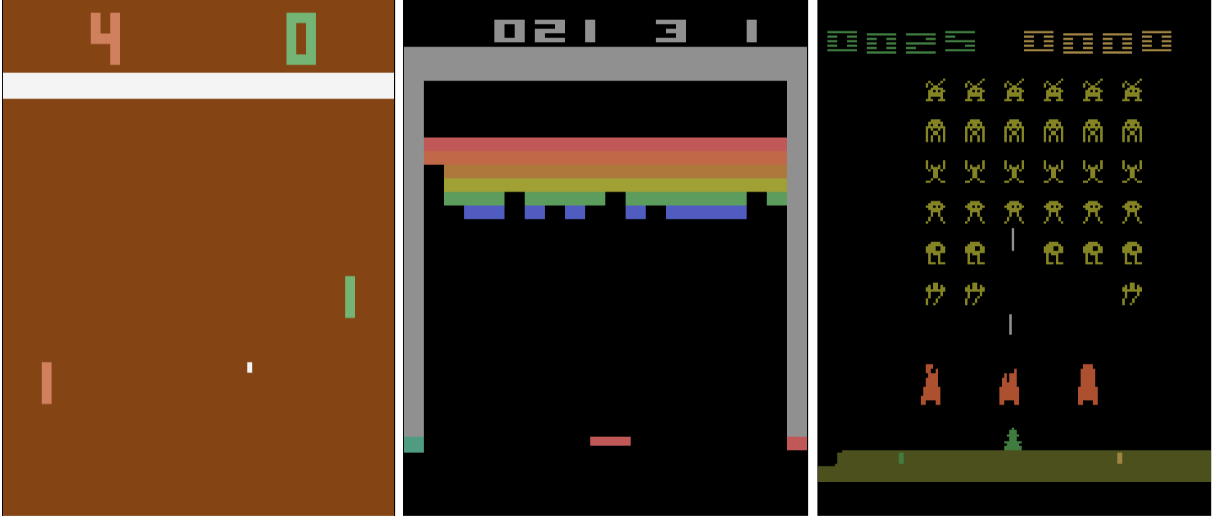
\includegraphics[width=3.2in]{fig_atari_games}
\caption{The three Atari games we used in this experiment: Pong (left), Breakout (middle), and Space
Invaders (right). Pong and Breakout are similar in that both use a paddle to hit a ball that bounces
in the game space. In Space Invaders, the player controls the ship at the bottom and aims to shoot
at all the other ships.}
\label{fig:atari}
\end{figure}

To gather human data in a principled, programmatic way, we implemented a task for workers on Amazon
Mechanical Turk (AMTurk), which is an online service where people can do tasks in exchange for
payment. For our AMTurk task, we had players play three of the Atari games: Pong, Breakout, and
Space Invaders. Figure~\ref{fig:atari} shows example screenshots of the three respective games.

We selected these three for several reasons. First, they are all commonly used as benchmarks
for DQN agents; the original paper that introduced DQN used these three
games~\cite{mnih-atari-2013}. Second, Pong and Breakout are similar because players control a
paddle and can move it in one axis (vertically for Pong, horizontally for Breakout) and have to
hit a moving, bouncing ball. Both games require skillful coordination to hit the
ball at the correct locations and momentum to get the balls to go in desired directions.
Consequently, Pong and Breakout may test the effect of transfer learning, which we can evaluate by
checking the game performances of those players on Pong with or without Breakout experience (so long
as we have sufficient players to reduce the variance with few players). Finally, Space Invaders is a
game that DQN performs reasonably well on, but still often loses to human players, and requires
long-term strategy. It might be worthwhile to start exploring the question as to whether human data
can improve DQN's performance on Space Invaders.

For the AMTurk experiment, each player was assigned one of the six possible game orderings to 
evaluate transfer learning. The players played each game for exactly ten minutes. To motivate
the players to play and get high scores (and to avoid just letting the timer run out without doing
anything) we set three payment thresholds based off of performance. For each game, players earned
\$1.00, \$1.50, and \$2.00 for clearing the first, second, and third thresholds, respectively. All
thresholds were based off of game scores. For instance, Breakout's thresholds were set at 5, 30, and
90 points for one game episode. The first two thresholds are easy enough so that almost all new
players can reach them, while the third requires some additional skill and is attainable only for
fast learners or experienced players.

We told the players which controls to use (the four arrow keys, plus the space bar), but did not
tell them what they did, with the exception of telling them that the space bar in Breakout allowed
the ball to appear. We did this because a pilot run indicated that confusion among the space bar was
a top issue.

We also made the players answer various survey questions to collect qualitative data. We had a set
of post-game questions that players had to answer right after they played a game. The template was:

\begin{itemize}
    \item A Likert question: \emph{I played well.}
    \item A Likert question about a game-specific strategy:
    \begin{itemize}
        \item Pong: \emph{It is a good strategy to try and make the ball take an angled path towards the opponent.}
        \item Breakout: \emph{It is a good strategy to try and clear the board by eliminating one row at a time.}
        \item S.I.: \emph{It is a good strategy to try and eliminate ships in one column before moving on to another column.}
    \end{itemize}
    \item (Free resp.) \emph{What was the final strategy you decided on?}
    \item (Free resp.) \emph{Was there anything from a previous game in this HIT\footnote{A HIT in AMTurk stands
    for ``Human Intelligence Task.''} that helped?}
\end{itemize}

The purpose of the game-specific Likert scale question is to get the players to think about good
general strategies for that game and also to make it easier for them to answer the free response
questions. All Likert questions were on a scale of five: strongly disagree, disagree, undecided,
agree, strongly agree.

This template of post-game survey questions was asked directly after a game, so players did the
following in succession: Game 1, post-game survey, Game 2, post-game survey, Game 3, post-game
survey, and then finalized their task with some general survey questions at the end. At the very
end, we ask the players if they think they now knew effective strategies for all three games
(True/False scale) and how they would rank their level of expertise in each game (novice,
intermediate, expert).  Our final question explicitly asks them if they thought they had developed
good strategies to play all three games. We discuss our results in Section~\ref{ssec:human_results}.

\subsection{Neural Network Classifier}\label{ssec:nn_experiment}

In active reinforcement learning, an \emph{exploration policy} is necessary because the agent needs
to explore the state space to learn an optimal policy. While it does so, it balances exploration
(trying new actions to reach new states) with exploitation (taking optimal actions according to
estimated state-action values). As reported in~\cite{mnih-dqn-2015}, the DQN algorithm follows a
$(1-\epsilon)$-greedy policy during training. This means the agent selects actions at random with
probability $\epsilon$, and follows the optimal action with probability $1-\epsilon$. Their
algorithm initialized $\epsilon=1$, and gradually reduced it to 0.1 over the first one million
frames, and then fixed it at 0.1 thereafter. The reason for high $\epsilon$ at the beginning is so
that the agent can sufficiently explore the state space, which is a requirement for Q-learning to
converge to the optimal policy.

Humans, however, do not generally perform random actions when first starting to play a game (i.e.,
during the ``exploration phase''). It would therefore be interesting to see what would happen to the
DQN agent during training if the $\epsilon$ cases correspond to actions that a \emph{human} would
most likely take (rather than being a random action). If a human can quickly learn how to play a
game well, then the actions he or she takes might help a DQN agent to converge to optimal policies
faster.

To pick an action that a human would likely take, we train a classifier that takes a downsampled
game frame as input and provides a ranking of actions as output (we only work with the highest
probability action). We use convolutional neural networks (CNNs) as our classifier due to their
strong performance on other image classification tasks.  The game log from the AMTurk experiments
provide the training data since it provides a record of all game frames encountered, along with the
corresponding keystrokes from the player. The CNN we design is based on the CNN
from~\cite{mnih-atari-2013}. It takes an $(84\times 84)$ grayscale image as input. The first hidden
layer convolves 16 $8\times 8$ kernels with stride size 4, then applies max-pooling and the
rectifier nonlinearity. The second hidden layer convolves 32 $4\times 4$ kernels with stride size 2,
then applies max-pooling and the rectifier nonlinearity. The third (and final) hidden layer is fully
connected and has 256 rectifier units. The output layer is a fully connected linear layer with a
single output for each valid action; the number of valid actions varies depending on the game.

Due to time and resource constraints, we only train a CNN for recognizing human actions from game
frames of the Space Invaders game, leaving Breakout and Pong frame-action classification for future
work. Space Invaders has six actions: nothing, fire, move-left, move-right, fire-move-left, and
fire-move-right. We describe our results in Section~\ref{ssec:nn_results}. We did not use this
classifier for training DQN, again due to time constraints, but our classifier is publicly available
\footnote{\url{https://github.com/DanielTakeshi/CS-287-Final-Project}} and it is straightforward to
incorporate it in Nathan Sprague's DQN
implementation\footnote{\url{https://github.com/spragunr/deep_q_rl}}.


%%%%%%%%%%%%%%%%%%%%%%%%%%%%%%%%%%%%%%%%%%%%%%%%%%%%%%%%%%%%%%%%%%%%%%%%%%%%%%%%
\section{Results}\label{sec:results}

\subsection{Human Experiment Results}\label{ssec:human_results}

\textbf{I think I'm good up to here.}

\begin{figure}[t]
\centering
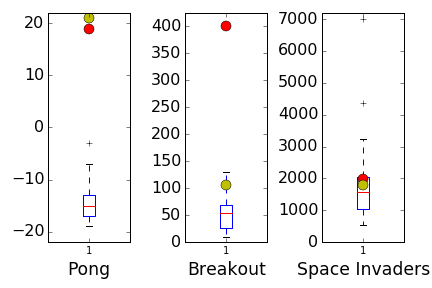
\includegraphics[width=3.2in]{fig_boxplots_human_results.png}
\caption{This displays boxplots of our 34 human players' results on the three games, with scores on
the $y$-axis. The boxes cover the 25th through 75th percentiles, with the median indicated by the
line in the box, and the whiskers go out to the minimum of the maximum element, or 1.5 times the
IQR of the data. The red dot is the \emph{average} DQN score for that game, and the yellow dot is
the author's \emph{average} score. Among all three plots, there are only three outliers. One is from
Pong, where one player lost 21-18 and therefore scored -3, and the other two are from Space
Invaders, where two different players scored 4370 and 7015 (!) points.}
\label{fig:human_results}
\end{figure}

We deployed our experiment on AMTurk in small sets, so as to not overload our server. We got a total
of \textbf{TODO} responses, which is less than our goal of 120, and in future work we plan on
finishing all 120.

First, we report on the raw scores players got. In Figure~\ref{fig:human_results}, we present three
boxplots of the players' \emph{highest} scores, for each of the three games. We also compare this
with the average DQN score (from the Nature paper), and the average score of the first author. (The
reason for using the highest of the players' scores is that they only have ten minutes, to provide a
reasonably fair comparison.) \textbf{TODO I might have to clarify this a bit.} We see that Pong was
especially difficult for the players. The score of Pong is calculated as the player score subtracted
from the computer score, so the scores range from $-21$ (i.e., losing 21 to 0) to $+21$. Breakout
was also difficult for them. A common complaint about Pong and Breakout was that the controls were
too difficult. Doing well in those games requires solid coordination in the controls, plus knowing
how to hit the balls diagonally. Breakout requires a fast reaction time, which is generally not a
problem for computer players. With Space Invaders, our players had a relatively easier time with the
controls, and consequently, were able to perform better, with our better players exceeding the
performance of DQN.

\begin{figure}[t]
\centering
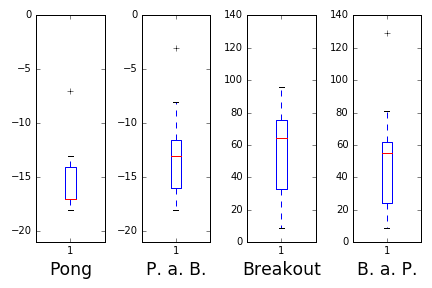
\includegraphics[width=3.2in]{fig_boxplots_transfer_learning}
\caption{This displays boxplots of humans playing Pong and Breakout with various orderings to test
the effect of transfer learning. Legend: ``Pong'' means playing Pong without having previously
played Breakout, ``P.a.B'' means playing Pong (a)fter (B)reakout, ``Breakout'' means playing
Breakout without having previously played Pong, and ``B.a.P.'' means playing Breakout (a)fter
(P)ong. The two Pong plots are scaled so that they have the same $y$-axis to facilitate comparison;
a similar case holds for the Breakout plots. Note that for these results, the ordering of Space
Invaders is irrelevant.}
\label{fig:human_transfer}
\end{figure}

\textbf{TODO discuss transfer learning, briefly}

We also received some interesting comments about the game. Here is a sampling of them (all from
different players, and non-edited):

\begin{itemize}
    \item (Pong) \emph{my strategy during this game was an utter disaster throughout the entire
    phase of play.}
    \item (Pong) \emph{Breakout helped learn how to hit the ball at an angle}
    \item (Breakout) \emph{Try to chip out one column then get the ball to go up the column and
    bounce around the top, hitting all the high point blocks}
    \item (Space Invaders) \emph{Eliminate most off the lowest aliens first, then concentrate on an
    outer column}
    \item (All games) \emph{If there were a way to have better contorl of the paddle, I would try to
    hit more angular shots in the PONG game. The Atari paddle controller on the old 2600 system made
    this easily possible. The keyboard controls show weakness [...]}
\end{itemize}

It is indeed problematic that controls were an issue, but it is difficult to get around that.

\subsection{Neural Network Experiment Results}\label{ssec:nn_results}

Our CNN is implemented and trained using CAFFE~\cite{caffe}.

\textbf{TODO try to get ANYTHING up here!}

Due to lack of computational power at our disposal, we were unable to run the experiments for as
long as we wished.


%%%%%%%%%%%%%%%%%%%%%%%%%%%%%%%%%%%%%%%%%%%%%%%%%%%%%%%%%%%%%%%%%%%%%%%%%%%%%%%%
\section{Conclusions and Future Work}\label{sec:conclusions}

\textbf{TODO elaborate on the importance of the results, once I get them!} 

Straightforward directions for future work include continuing the Amazon Mechanical Turk experiments
on more human participants, testing on other Atari games, and identifying which DQN settings to use
to maximize the benefit of human data. Some more elaborate extensions of this work might involve
running Q-Learning on the human data itself to see if the Q-Learner's policy is as good as what DQN
learned, and investigating inverse reinforcement learning to propose a pseudo-reward function that
explains people's behavior in their exploration stages.

%%%%%%%%%%%%%%%%%%%%%%%%%%%%%%%%%%%%%%%%%%%%%%%%%%%%%%%%%%%%%%%%%%%%%%%%%%%%%%%%
\section*{Acknowledgments}

We thank Andrew Liu for setting up the Amazon Mechanical Turk experiment.


%%%%%%%%%%%%%%%%%%%%%%%%%%%%%%%%%%%%%%%%%%%%%%%%%%%%%%%%%%%%%%%%%%%%%%%%%%%%%%%%

\addtolength{\textheight}{-12cm}
% This command serves to balance the column lengths on the last page of the document manually. It
% shortens the textheight of the last page by a suitable amount.  This command does not take effect
% until the next page so it should come on the page before the last. Make sure that you do not
% shorten the textheight too much.

\bibliographystyle{IEEEtran}
\bibliography{Daniel_Seita_Final_Paper_CS287}

% Daniel: This was their old table code.
%\begin{table}[h]
%\caption{An Example of a Table}
%\label{table_example}
%\begin{center}
%\begin{tabular}{|c||c|}
%\hline
%One & Two\\
%\hline
%Three & Four\\
%\hline
%\end{tabular}
%\end{center}
%\end{table}

% Daniel: This was their old figure code.
%\begin{figure}[thpb]
%\centering
%\framebox{\parbox{3in}{We suggest that you use a text box to insert a graphic (which is ideally a
%300 dpi TIFF or EPS file, with all fonts embedded) because, in an document, this method is somewhat
%more stable than directly inserting a picture.  }}
%%\includegraphics[scale=1.0]{figurefile}
%\caption{Inductance of oscillation winding on amorphous
%magnetic core versus DC bias magnetic field}
%\label{figurelabel}
%\end{figure}


\end{document}
